% ---------------------------------------------------------------------
% HEADER
% Formålet med å legge header til et eget dokument er å garantere at
% oppsettet av dokumentene er likt for alle løsningsforslagene.
% I headeren skjer følgende:
% (1) Dokumentet blir startet
% (2) Pakker blir importert
% ---------------------------------------------------------------------
% ---------------------------------------------------------------------
% HEADER
% Formålet med header er å importere de samme pakkene i alle dokumentene.
% ---------------------------------------------------------------------

% Sett opp dokumentet. Her kan 'twoside' brukes for printing
\documentclass[12pt, a4paper]{article}

% Vi trenger utf-8 for å bruke norske bokstaver: Æ, Ø, Å
\usepackage[utf8]{inputenc}

% Vi setter babel til norsk, da får dokumentegenskaper norske titler
\usepackage[norsk]{babel}

% For å kunne bruke grafikk
\usepackage{graphicx}
\newcommand{\figwidth}{0.75}

% Matematikkpakker fra AMS - American Mathematical Society
\usepackage{amsmath, amsthm, amsfonts, amssymb, mathtools}

% For eventuelle linker, e.g. \href{URL}{text}
\usepackage{hyperref}

% For headers og footers med eventuell logo
\usepackage{fancyhdr}

% Sett marginer manuelt
\usepackage[top = 3cm, left = 3cm, right = 3cm, bottom = 3cm]{geometry}

% For enkle lister, nyttig for oppgave a), b), c), ...
\usepackage[sharp]{easylist}

% Dersom flere kolonner er ønskelig i deler av dokumentet
\usepackage{multicol}

% For luft mellom paragrafer
\usepackage{parskip}

% For logikk assosiert med logoer
\usepackage{ifthen}

% For å finne totalt antall sider
\usepackage{lastpage}

% Annet
\usepackage{enumitem}

\usepackage{polynom}% Polynomer
\polyset{style=C, div=:}

\usepackage{systeme}% Likningssystemer

% Kan brukes når noe stryker ut noe, f.eks 1/n * n, her kan man ta \frac{1}{\cancel{n}} * \cancel{n}
\usepackage{cancel}



% ---------------------------------------------------------------------
% DOKUMENTVARIABLER
% ---------------------------------------------------------------------
\newcommand{\fagkode}{S2}
\newcommand{\semesteraar}{høsten 2016}
\newcommand{\forfatter}{Tommy O.}
\newcommand{\dokumenttittel}{Løsningsforslag -- Eksamen \fagkode, \semesteraar}


% Set til 'true' og oppgi logo dersom du vil bruke en logo
\newboolean{bruklogo}
\setboolean{bruklogo}{true}
\newcommand{\logonavn}{figs/metis_akademiet_privatistskole_doclogo.png}

% ---------------------------------------------------------------------
% SETUP
% Formålet med å legge setup til et eget dokument å garantere at headers,
% footers, og øverste del av dokumentet er likt for alle
% løsningsforslagene.
% ---------------------------------------------------------------------
% ---------------------------------------------------------------------
% HEADER
% Formålet med setup er at dokumentene ser rimelig like ut.
% ---------------------------------------------------------------------


% ---------------------------------------------------------------------
% Alternativ font. Kommentert ut fordi Computer Modern (default) er pen
%\usepackage{kmath,kerkis}
%\usepackage[T1]{fontenc}
% ---------------------------------------------------------------------


% ---------------------------------------------------------------------
% Sett opp headers og footers
\ifthenelse{\boolean{bruklogo}}{
% Dersom logo skal brukes, sett logoen oppe til høyre med bredde 4 cm
	\rhead{\includegraphics[width=3.5cm]{\logonavn}}
}{
% Dersom logo ikke skal brukes, sett tom header
	\rhead{}
} 
\rfoot{\thepage}
\cfoot{}
\lhead{}
\lfoot{{\scriptsize Forbedringsforslag? Bidra på \url{https://github.com/tommyod/matte_eksamener_VGS}.}}
\renewcommand{\headrulewidth}{0pt}
% ---------------------------------------------------------------------


% ---------------------------------------------------------------------
% To streker under svaret
\def\answer#1{\underline{\underline{#1}}}
% ---------------------------------------------------------------------


% ---------------------------------------------------------------------
% Start selve dokumentet
% ---------------------------------------------------------------------

\begin{document}
\pagestyle{fancy}
{\bfseries \Large \dokumenttittel} \\
{ \footnotesize Laget av \forfatter 
	\hfill Sist oppdatert: \today 
	\hfill Antall sider: \pageref*{LastPage}}
\hrule
\vspace{1em}
\begin{center}
\fbox{\fbox{\parbox{.90\textwidth}{
	Dette dokumentet er open-source;
	alle kan bidra til å gjøre det bedre.
	Dersom du finner skrivefeil, matematiske feil, eller ser at forklaringene kan være bedre: ikke nøl med å sende inn en endring. 
	Du kan finne siste versjon, og bidra, på GitHub, se:
	\url{https://github.com/tommyod/matte_eksamener_VGS}
}}}
\end{center}


% ---------------------------------------------------------------------
% DOKUMENTSTART - Skriv løsningsforslaget nedenfor
% ---------------------------------------------------------------------	

\section*{Del 1 - uten hjelpemidler}
\subsection*{Oppgave 1}
\begin{easylist}[enumerate]
	\ListProperties(Style2*=,Numbers=a,Numbers1=l,FinalMark={)})
	# Vi skal derivere $f(x) = x^3 - 5x$, og vi kommer til å få bruk for reglene $\left(ax^n\right)' = anx^{n-1}$ og $\left(f(x) + g(x)\right)' = f'(x) + g(x)$. 
	Når vi deriverer får vi $f'(x) = \answer{3x^2 - 5}$.
	
	# Vi skal derivere $g(x) = 5(x^2 + 1)^7$. 
	Her må vi bruke kjerneregelen, og vi setter $u = x^2 + 1$ som kjerne. Da er $u' = 2x$, og vi får $f(u) = 5u^7$ slik at $f'(u) = 35 u^6 u' = 35 \left(x^2 + 1\right)^6 \left(2x\right) = \answer{70x \left(x^2 + 1\right)^6}$.
	
	# Vi skal derivere $h(x) = \frac{e^x}{e^x + 1} = e^x \left(e^x + 1\right)^{-1}$.
	Legg merke til at vi skriver om brøken til faktorer slik at vi kan bruke produktregelen $(uv)' = u'v + uv'$, ettersom produktregelen er enklere å huske enn brøkregelen.
	Da får vi følgende utregning:
	\begin{align*}
	h'(x) &= \left( e^x \right)' \left(e^x + 1\right)^{-1} + e^x \left( \left(e^x + 1\right)^{-1} \right)' \\
	&= e^x \left(e^x + 1\right)^{-1} + e^x (-1) \left(e^x + 1\right)^{-2} e^x \\
	&= \frac{e^x}{e^x + 1} -\frac{\left(e^x\right)^2}{\left(e^x + 1\right) \left(e^x + 1\right)} \\
	&= \frac{e^x\left(e^x + 1\right) - \left(e^x\right)^2}{\left(e^x + 1\right)^2} \\
	&= \answer{\frac{e^x}{\left(e^x + 1\right)^2}}
	\end{align*}
\end{easylist}

\subsection*{Oppgave 2}
\begin{easylist}[enumerate]
	\ListProperties(Style2*=,Numbers=a,Numbers1=l,FinalMark={)})
	# Oppgaven går ut på å løse følgende likning for $x$:
	\begin{equation*}
	\frac{3x}{x-2} = \frac{x^2}{x^2 - 4}
	\end{equation*}
	Vi begynner med å finne fellesnevner. Gang venstre side med $(x+2)$ og bruk at $(x-2)(x+2) = x^2 - 4$ til å skrive likningen som :
	\begin{equation*}
	\frac{3x(x+2)}{x^2 - 4} = \frac{x^2}{x^2 - 4}
	\end{equation*}
	Gang så begge sider med $(x^2 - 4)$ for å bli kvitt nevneren. Vi løser likningen $3x(x+2) = x^2$ slik
	\begin{equation*}
	3x(x+2) = x^2 \Rightarrow 2x^2 + 6x = 0 \Rightarrow 2x(x + 3) = 0
	\end{equation*}
	Løsningen er $\answer{x = 0 \ \vee \ x = -3}$.
	
	# Vi skal løse likningen:
	\begin{equation*}
	\ln \left( x^2 + 2x - 14\right) = 0
	\end{equation*}
	Vi må huske at $ \ln (y) = 0 \Rightarrow y = 1$.
	Med andre ord må vi løse følgende:
	\begin{equation*}
	\ln \left( x^2 + 2x - 14\right) = 0 \Rightarrow x^2 + 2x - 14 = 1
	\end{equation*}
	Bruker ABC-formelen\footnote{For mer om ABC-formelen, se \url{http://www.purplemath.com/modules/quadform.htm}} og får løsningene  $\answer{x = -5 \ \vee \ x = 3}$.
\end{easylist}

\subsection*{Oppgave 3}
I denne oppgaven skal vi se på følgende funksjon:
\begin{equation*}
f(x) = x^3 - 6x^2 + 32
\end{equation*}
\begin{easylist}[enumerate]
	\ListProperties(Style2*=,Numbers=a,Numbers1=l,FinalMark={)})
	# Divisjonen $f(x) : (x+2)$ går opp dersom $\frac{f(x)}{(x+2)} = p(x)$, der $p(x)$ er et polynom. Da må vi ha $\frac{f(x)}{(x+2)} = p(x) \Rightarrow f(x) = (x+2) p(x)$. Siden høyre side er lik null når $x = -2$ må det også gjelde for venstre side, altså må $\answer{f(-2) = 0}$. Dette kan vi sjekke at stemmer slik:
	\begin{equation*}
	f(-2) = (-2)^3 - 6(-2)^2 + 32 = -8 -24 +32 = 0
	\end{equation*}
	
	# Utfør polynomdivisjonen $f(x):(x+2) = p(x) = x^2 - 8x + 16$. Vi kan faktorisere $p(x)$ ved hjelp av ABC-formelen slik at $p(x) = x^2 - 8x + 16 =  (x-4)^2$. Med andre ord er $f(x) = (x+2)(x-4)^2$ og nullpunktene har $x = 4$ og $x = -2$. Nullpunktene er da $(4, f(4)) = \answer{(4, 0)}$ og  $(4, f(-2)) = \answer{(-2, 0)}$.
	
	# For å finne topp- og bunnpunkter deriverer vi $f(x)$ og får $f'(x) = 3x^2 - 12x$.
	Dersom $f'(x^*) = 0$ i et punkt $x^*$ er punktet $\left(x^*, f\left(x^*\right)\right)$ enten et toppunkt, bunnpunkt eller terrassepunkt(også kalt sadelpunkt). 
	Vi løser $f'(x) = 3x^2 - 12x = 0$ og får $x_1 = 0$ og $x_2 = 2$. For å karakterisere punktene kan vi se på den dobbelderiverte $f''(x) = 6x - 12$.
	## I punktet $x_1 = 0$ har vi at $f(x_1) = 32$. Ettersom $f''(0) < 0$ er dette et toppunkt. \answer{Punktet $(0, 32)$ er et toppunkt}.
	## I punktet $x_2 = 4$ har vi at $f(x_2) = 0$. Ettersom $f''(4) > 0$ er dette et bunnpunkt. \answer{Punktet $(4, 0)$ er et bunnpunkt}.
	
	# Generelt oppstår et vendepunkt når den dobbelderiverte skrifter fortegn. 
	Vi ser når $f''(x) = 6x - 12$ skifter fortegn. Dette skjer når $x = 2$. Punktet $\left(2, f(2)\right) = \answer{\left(2, 16\right)}$ er altså et vendepunkt.
	
	# Funksjonen er skissert i figur \eqref{fig:oppgave3}. 
	Den deriverte og dobbelderiverte er også tegnet inn.
	Med informasjon om nullpunkter, topp- og bunnpunkter samt vendepunkt er det mulig å lage en god skisse uten digitale hjelpemidler.
	
	\begin{figure}[th!]
		\centering
		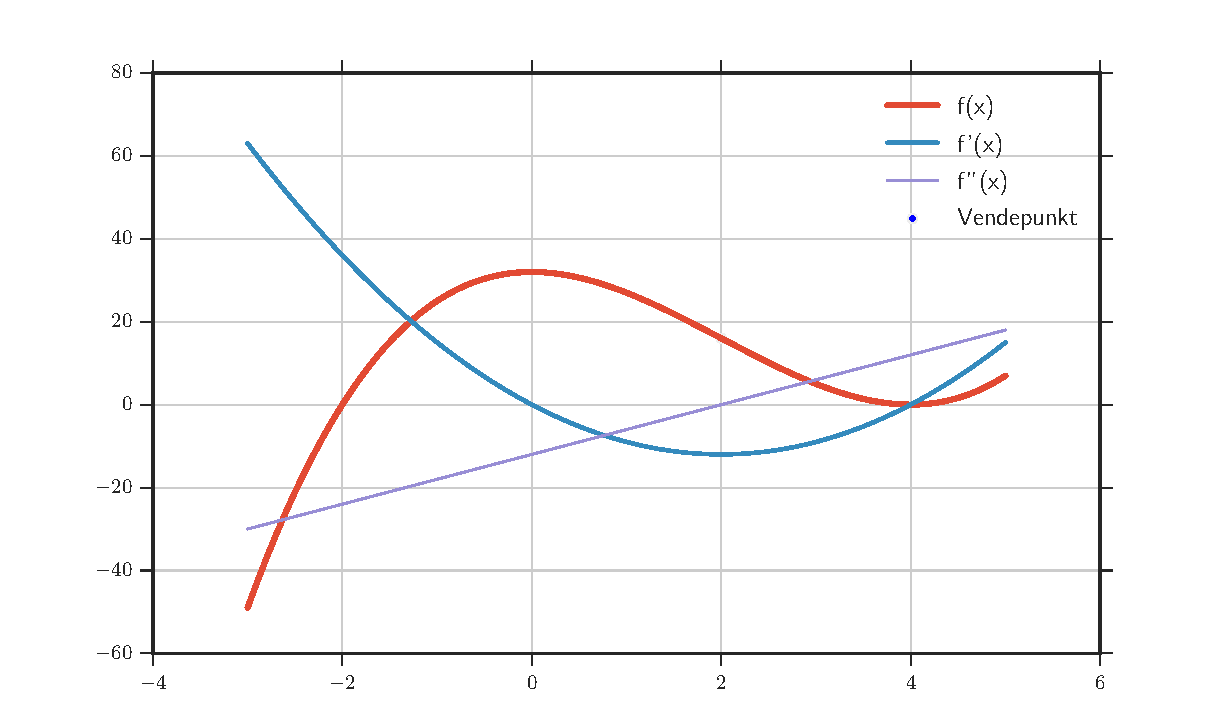
\includegraphics[width=0.9\linewidth]{figs/oppgave3.pdf}
		\caption{Skisse av $f(x) = x^3 - 6x^2 + 32$ til oppgave 3e.}
		\label{fig:oppgave3}
	\end{figure}
\end{easylist}


\subsection*{Oppgave 4}
\begin{easylist}[enumerate]
	\ListProperties(Style2*=,Numbers=a,Numbers1=l,FinalMark={)})
	# Likningssystemet kommer fra følgende observasjoner
	\begin{align*}
	\text{Likning 1: }&K(10) = 3000\Rightarrow & 100a + 10b + c = 3000 \\
	\text{Likning 2: }&K(20) = 8000 \Rightarrow & 400a + 20b + c = 8000 \\
	\text{Likning 3: }&K'(10) = 350 \Rightarrow & 20a + b = 350 
	\end{align*}
	Husk at ``grensekostnadene'' betyr bare ``derivert av kostnadsfunksjonen.''
	# Ta likning 2 minus likning 1. Vi får $300a + 10b = 5000$. 
	Sammen med likning 3 er dette et likningssystem med 2 likninger og 2 ukjente. 
	Løs systemet og finn at $\answer{a = 15}$ og $\answer{b = 50}$. 
	Finn så $\answer{c = 1000}$ ved innsetting i likning 1 eller 2.
\end{easylist}

\subsection*{Oppgave 5}
\begin{easylist}[enumerate]
	\ListProperties(Style2*=,Numbers=a,Numbers1=l,FinalMark={)})
	# Summeformelen som det refereres til her er:
	\begin{equation}
	\label{eqn:summeformel}
	S_n = \frac{a_1 + a_n}{2} \cdot n
	\end{equation}
	I vårt tilfelle er $a_1 = 1$ og $a_n = n$, vi setter dette inn i likning \eqref{eqn:summeformel} ovenfor og får følgende:
	\begin{equation*}
	S_n = \frac{a_1 + a_n}{2} \cdot n = \frac{1 + n}{2} \cdot n = \answer{\frac{\left(1+n\right)n}{2}}
	\end{equation*}
	
	# På figuren ser vi at arealet er lik er lik $2 \times \left( 1+2+3+ \dots +n \right)$. 
	Samtidig ser vi at arealet er lik bredde ganget med høyde, som blir $(n+1)n$. 
	Vi har altså følgende likninger:
	\begin{align*}
	\text{areal} &= 2 \times \left( 1+2+3+ \dots +n \right)  \\
	\text{areal} &= (n+1)n 
	\end{align*}
	Dersom vi nå setter $\text{areal} = \text{areal}$ får vi følgende:
	\begin{equation*}
	1+2+3+ \dots +n = \frac{\left(1+n\right)n}{2}
	\end{equation*}
	Som er samme svar som forrige deloppgave. 
	Det kan være lurt å sette inn $n = 1,2,3$ og sjekke at det stemmer for enkle tilfeller.
\end{easylist}

\subsection*{Oppgave 6}
\begin{easylist}[enumerate]
	\ListProperties(Style2*=,Numbers=a,Numbers1=l,FinalMark={)})
	# Vi vet at \answer{summen av sannsynlighetene må være lik 1.} Skrevet litt mer matematisk:
	\begin{equation*}
	\sum_{t \in X}P(X = t) = 1
	\end{equation*}
	Derfor får vi $0,1 + 0,3 + 0,2 + p = 1$, og da må vi ha $p = 0,4$.
	
	# Definisjonen av $\operatorname{E}(X)$ er $\operatorname{E}(X) = \sum_{t \in X}P(X = t)t$, og vi får
	\begin{equation*}
	\operatorname{E}(X) = \sum_{t \in X}P(X = t)t =  0,1(r) + 0,3(-1) + 0,2 (0) + 0,4(2) = 1
	\end{equation*}
	Fra likningen ovenfor ser vi at $\answer{r = 5}$.
	
	# Dersom $r = -5$ kan vi bruke samme tankegang som i forrige deloppgave til å regne ut at  $\answer{\operatorname{E}(X) = 0}$. Generelt er likningen for varians gitt ved:
	\begin{equation*}
	\operatorname{Var}(X) = \sum_{t \in X}P(X = t)(t - \operatorname{E}(X))^2 
	\end{equation*}
	Ettersom $\operatorname{E}(X) = 0$ får vi en rimelig enkel utregning:
	\begin{equation*}
	\operatorname{Var}(X) = \sum_{t \in X}P(X = t)t^2 =0,1(-5)^2 + 0,3(-1)^2 + 0,2(0)^2 +0,4(2)^2 = \answer{4,4}
	\end{equation*}
\end{easylist}


\subsection*{Oppgave 7}
\begin{easylist}[enumerate]
	\ListProperties(Style2*=,Numbers=a,Numbers1=l,FinalMark={)})
	# Vi har overskudd dersom inntekten er større enn kostnaden(utgiften). 
	Da må vi ha at $I(x) - K(x) > 0$. Dette skjer når den røde linjen er større enn den blå,
	altså når $\answer{x \in \langle 100, 400 \rangle}$. 
	En alternativ skrivemåte for dette intervallet er $100 < x < 400$.
	
	# Grensekostnaden $K'(x)$ er den deriverte av kostnaden $K(x)$.
	Funksjonen $h$ er tangenten til $K(x)$ i punktet $x=100$.
	En tangent i et punkt matcher funksjonsverdien og den deriverte, så vi vet at 
	tangenten derivert er lik funksjonen derivert i punktet.
	Vi leser at $g(x) = 62,5x +3850$, så da er $g'(x) = K'(x) = \answer{62,5}$.
	
	# Overskuddet $O(x) = I(x) - K(x)$ er størst i punktet $B$. Da er $\answer{x = 250}$.
	Bedriften må altså produsere og selge 250 enheter for størst overskudd.
	
\end{easylist}


\subsection*{Oppgave 8}
Her holder det å se på forventningsverdien $\mu = \operatorname{E}(X)$ og standardavviket $\sigma = \operatorname{SD}(X)$ i begge tilfellene.
\begin{easylist}[itemize]
	\ListProperties(Space*=-.5em, Space=-.5em)
	# På flervalgsprøven er $\mu = 32 \frac{1}{3} \approx 10,66$. Den eneste figuren som har normalfordeling med forventningsverdi i nærheten av $10$ er \answer{\textbf{figur D}}.
	# I frø-scenarioet er $\mu = 100 \frac{8}{10} = 80$. Det er 2 figurer som har forventningsverdi i nærheten av $80$: \textbf{figur A} og \textbf{B}. Vi ser på standardavviket, og regner ut at  $\operatorname{SD}(X) = \sqrt{n p (1- p)} = \sqrt{100 0,8 (1- 0,8)} = \sqrt{16} = 4$. Dersom $X$ er normalfordelt vet vi at $\sim 68 \%$ ligger innenfor $\pm \sigma$ (ett standardavvik). Mer enn halvparten av arealet skal altså ligge i området $80 \pm 4$, og da må \answer{\textbf{figur A}} være riktig svar.
\end{easylist}




\section*{Del 2 - med hjelpemidler}
\subsection*{Oppgave 1}
\begin{easylist}[enumerate]
	\ListProperties(Style2*=,Numbers=a,Numbers1=l,FinalMark={)})
	# La $h$ være høyden. Ettersom volumet skal være $800 \text{ liter} = 0,8 \text{ m}^3$ får vi likningen:
	\begin{equation*}
	x \times x \times h = 0,8 \Rightarrow h = \frac{0,8}{x^2}
	\end{equation*}
	Kostnaden er kostnader per flate ganget med flateområde. For de forskjellige flatene får vi derfor følgende kostnader:
	\begin{align*}
	\text{Bunn: }& x^2 \times 450 \\
	\text{Topp: }& x^2 \times 230 \\
	\text{Side: }& xh \times 230 
	\end{align*}
	Vi legger dette sammen for å finne den totalt kostnaden. Husk at det er 4 sider. 
	\begin{align*}
	K(x) &= \text{bunn} + \text{topp} + 4 \times \text{side} \\ 
	&= x^2 \times 450 + x^2 \times 230 + 4 \times xh \times 230 \\ 
	&= x^2 \times 450 + x^2 \times 230 + 4 \times x\left(\frac{0,8}{x^2}\right) \times 230 \\ 
	&= 450x^2 + 230 x^2 + \frac{736}{x} = \answer{680 x^2 + \frac{736}{x}}
	\end{align*}
	
	# Tegning av grafen finnes i figur \eqref{fig:oppgave1}.
	\begin{figure}[th!]
		\centering
		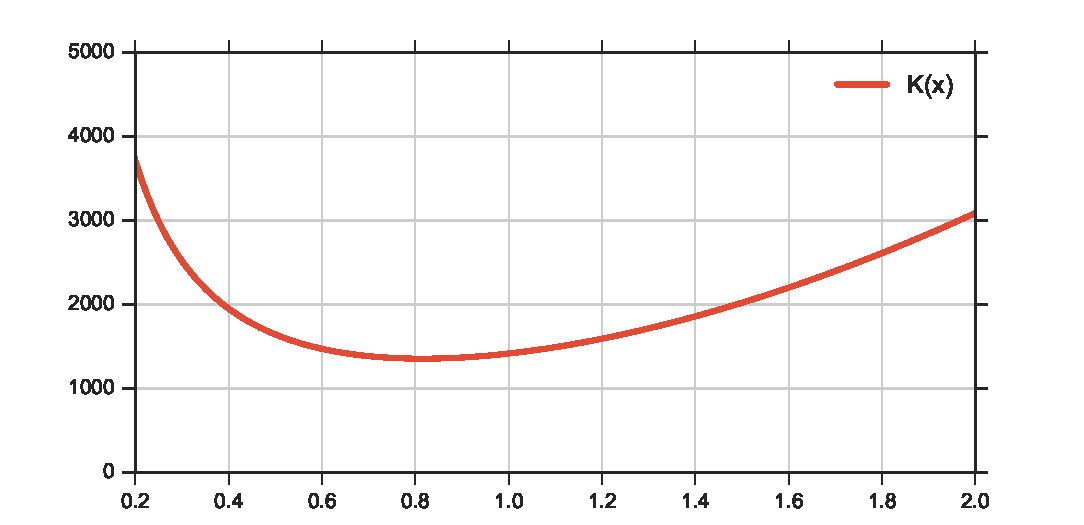
\includegraphics[width=0.9\linewidth]{figs/oppgave1.pdf}
		\caption{Skisse av $K(x) = 680x + \frac{736}{x}$ til oppgave 1b, del 2.}
		\label{fig:oppgave1}
	\end{figure}
	
	# Definer funksjonen som \texttt{K(x) = 680*x*x + 736/x} i Geogebra og skriv inn:\\
	\texttt{Min[K, 0, 2]} \\
	La oss kalle $x$-verdien som minimerer $K(x)$ for $x^*$, slik at $K(x^*) = \text{minimum}$.
	Svaret vi får fra Geogebra er $\answer{x^* \approx 0,815}$. Dersom vi ønsker flere desimaler kan vi gå på ``Innstillinger'' $\rightarrow$ ``Avrunding'' i hovedmenyen i Geogebra.
\end{easylist}

\subsection*{Oppgave 2}
\begin{easylist}[enumerate]
	Dette er et scenario styrt av binomisk fordeling.
	\ListProperties(Style2*=,Numbers=a,Numbers1=l,FinalMark={)})
	# Binomisk med $n = 10$ og $p = 0,52$. Åpne sannsynlighetskalkulatoren til Geogebra ved å trykke ``Vis'' $\rightarrow$ ``Sannsynlighetskalkulator.'' Les av $\answer{P(7 \leq X) \approx 0,2067}$.
	
	# Her har vi 2 muligheter:
	## Bruk binomisk (som i forrige oppgave) med $n = 100$ og $p = 0,52$. Da får vi $P(70 \leq X) = 0,0001900128 = \answer{0,0002}$ i Geogebra.
	## Vi kan approksimere (tilnærme) den binomiske fordelingen med normalfordeling dersom $np$ og $n(1-p)$ begge er minst lik 5.\footnote{Dette er en tommelfingerregel.} Bruk normalfordeling med 
	\begin{align*}
	\mu &= n p = 100 (0,52) = 52 \\
	\sigma &= \sqrt{np(1-p)} = \sqrt{100(0,52)(0,48)} \approx 4,996
	\end{align*}
	Vi setter dette inn i Geogebras sannsynlighetskalkulator under normalfordeling og får $P(69,5 \leq X) = 0.0002301956 \approx \answer{0.0002}$.
	Legg merke til heltallskorreksjonen. Å se på $P(X \geq 70)$ i en diskret fordeling må tilnærmes til $P(X \geq 69,5)$ i en kontinuerlig fordeling.
	
	# Vi har følgende hypoteser:
	\begin{align*}
	H_0 &: p = 0,52 \\
	H_1 &: p > 0,52 
	\end{align*}
	La $k$ være antall personer av $n = 100$ som består teoriprøven. 
	Den observerte verdien av $k$ er $k_{\text{obs}} = 60$. 
	$P$-verdien er sannsynligheten for å få $k \geq k_{\text{obs}}$ gitt at $H_0$ er er sann.
	Med andre ord er $P$-verdien sannsynligheten for at 60 personer eller flere består når $p = 0,52$.
	Vi bruker binomisk sannsynlighetskalkulator i Geogebra til å regne ut følgende:
	\begin{equation*}
	P\text{-verdi} = P(k \geq 60 | p = 0,52) = 0.0662296331 \approx 0.066
	\end{equation*}
	Ettersom $P$-verdien er større enn $0.05$ kan vi \answer{ikke forkaste $H_0$}.
\end{easylist}

\subsection*{Oppgave 3}
\begin{easylist}[enumerate]
	\ListProperties(Style2*=,Numbers=a,Numbers1=l,FinalMark={)})
	# Inntekten $I(p)$ er etterspørsel $x = E(p)$ ganget med prisen $p$.
	\begin{equation*}
	I(p) = E(p) \times p = \left(341 - p^2\right)p =  \answer{- p^3 + 341p}
	\end{equation*}
	
	# Vi må finne maksimum til $I(p) = - p^3 + 341p$.
	Dette er enkelt å gjøre for hånd, men vi kan bruke CAS slik som dette:\\
	\verb|I(p) := -p^3 + 341p, p > 0|\\
	Skriv deretter: \\
	\verb|NLøs[{I'(p) = 0}, {p}]| \\
	Prisen som gir høyest inntekt er \answer{$p = 10.66$}.
	
	
	# Vi vet at overskuddet er inntekt minus kostnad. Vi har en funksjon for inntekt,
	så vi trenger en funksjon for kostnad. 
	Fra figur \eqref{fig:oppgave3_2} ser vi at datasettet passer godt til lineær regresjon på formen $y = ax + b$. Vi kan lage regresjonslinje med kommandoen \texttt{RegPoly[ <Liste med punkt>, <Polynomgrad> ]} i Geogebra for polynomer av forskjellige grader.
	\begin{figure}[th!]
		\centering
		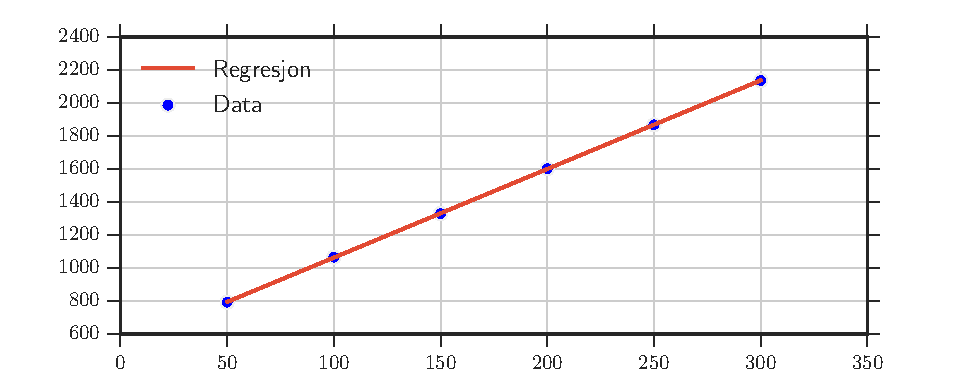
\includegraphics[width=0.9\linewidth]{figs/oppgave3_2_regr.pdf}
		\caption{Regresjonslinje $y = 5,37x +525,2$ for data i oppgave 3c, del 2.}
		\label{fig:oppgave3_2}
	\end{figure}
	Vi regner ut overskuddet slik:
	\begin{align*}
	O(p) &= I(p) - K(x) \\
	&= \left(- p^3 + 341p\right) - \left(5,37x +525,2\right) \\
	&= \left(- p^3 + 341p\right) - \left(5,37\left(341-p^2\right) +525,2\right) \\
	&= - p^3 + 341p - 1831,17 + 5,37p^2 - 525,2 \\
	&= - p^3 + 5,37p^2 + 341p - 2356,37 \\
	&\approx \answer{- p^3 + 5,37p^2 + 341p - 2356}
	\end{align*}
	
	# Definer funksjonen i Geogebra som \texttt{O(p)} (se figur \eqref{fig:oppgave3_3}) og skriv følgende:\\
	\texttt{Maks[O, 8, 16]}
	\\
	La $p^*$ være verdien som maksimerer $O(p)$. Svaret vi får er at overskuddet er størst i $p^* \approx 12,6$, og $O(p^*) \approx 792,77$.
	Oppgaven spør hvor mange enheter $x = E(p)$ som bedriften må produsere. Dette kan vi nå regne ut slik:
	\begin{equation*}
	x^* = E(p^*) = 341 - (12,6)^2 = 182,24 \approx \answer{182}
	\end{equation*}
	
	\begin{figure}[th!]
		\centering
		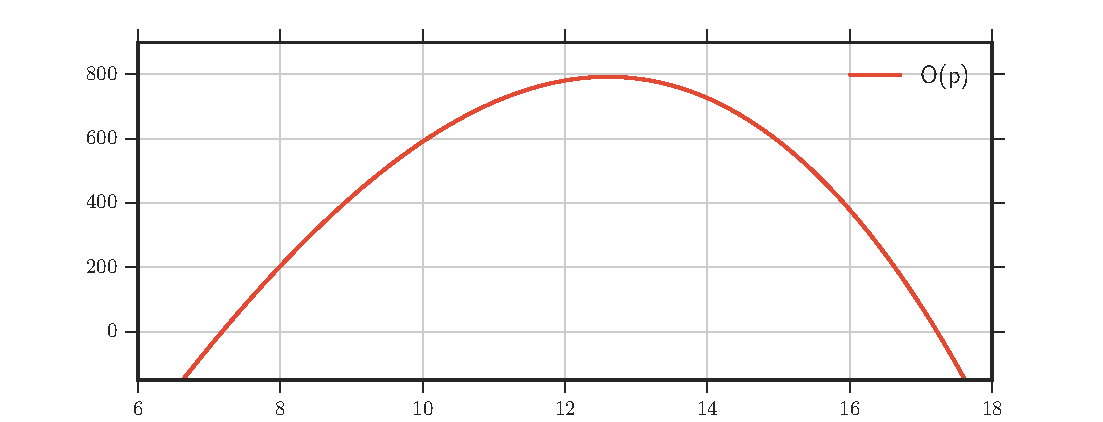
\includegraphics[width=0.8\linewidth]{figs/oppgave3_2_overskudd.pdf}
		\caption{Plot av $O(p)$ til oppgave 3d, del 2.}
		\label{fig:oppgave3_3}
	\end{figure}
\end{easylist}

\subsection*{Oppgave 4}
\begin{easylist}[enumerate]
	\ListProperties(Style2*=,Numbers=a,Numbers1=l,FinalMark={)})
	# Denne oppgaven kan selvsagt løses på flere måter, men la oss utvikle litt generell teori.
	La $L$ være lånebeløpet, $r$ være rentefaktoren, $t$ være terminbeløpet og $a$ være totalt antall år.
	I et annuitetslån er terminbeløpet konstant. Tabellen viser hvor mye
	en person skylder etter forskjellige år:
	\begin{center}
		\begin{tabular}{l|l|l}
			\textbf{År} & \textbf{Skyldig beløp} & \textbf{Pent uttrykk for skyldig beløp} \\ \hline
			1 & $L\times r - t$ & $L\times r - t$ \\
			2 & $\left(L\times r - t\right) \times r - t$ & $L^2 - tr -r$ \\
			3 & $\left( \left(L\times r - t\right) \times r - t  \right) \times r - t$ & $Lr^3 - tr^2 - tr - t$ \\
			$\vdots$ & $\vdots$ & $\vdots$ \\
			$a$ & $\dots$ & $Lr^a - t \sum_{i=0}^{a-1} r^i$ 
		\end{tabular}
	\end{center}
	I tabellen kan vi bruke litt algebra for å lage et pent uttrykk for skyldig beløp.
	Vi innser at dette pene uttrykket inneholder en geometrisk sum. 
	Etter $a$ år skal det skyldige beløpet være lik null. Vi får altså likningen:
	\begin{equation*}
	Lr^a - t \sum_{i=0}^{a-1} r^i = 0
	\end{equation*}
	Vi løser denne likningen for $t$ og bruker formelen for sum av geometrisk rekke til å skrive $\sum_{i=0}^{a-1} r^i$ som $ \frac{r^a-1}{r-1}$, vi får da denne formelen for $t$:
	\begin{equation}
	\label{renteformel}
	t = \frac{Lr^a(r-1)}{r^a-1}
	\end{equation}
	La oss sette inn $L = 100000$, $r = 1,024$ og $a = 25$ og løse:
	\begin{equation*}
	t = \frac{Lr^a(r-1)}{r^a-1} = \frac{100000\left(1,024\right)^{25}(1,024-1)}{\left(1,024\right)^{25}-1} \approx \answer{53657}
	\end{equation*}
	
	# Vi setter $t = 60000$ og løser likning \eqref{renteformel} for $r$.
	Dette kan vi gjøre ved å definere følgende i CAS i Geogebra: \\
	\texttt{a  := 25} \\
	\texttt{L := 1000000} \\
	\texttt{t := 60000} \\
	\texttt{Nløs[t = (L*r\textasciicircum a*(r-1))/(r\textasciicircum a-1), r]} \\
	$\rightarrow$ \texttt{r = 1.033973455474} \\
	Svaret blir $\answer{r \approx 1,034}$.
	Det kan være lurt å dobbelsjekke ved å sette $r = 1,034$ inn i likning \eqref{renteformel}. Vi får da at $t = 60017$, noe som er veldig nært 60000.
	
	# Skriv følgende i CAS i Geogebra: \\
	\texttt{L := 1000000} \\
	\texttt{r := 1.024} \\
	\texttt{t := 60000} \\
	\texttt{Nløs[t = (L*r\textasciicircum a*(r-1))/(r\textasciicircum a-1), a]} \\
	$\rightarrow$ \texttt{a = 21.53880422748} \\
	Svaret blir $\answer{a \approx 21.54}$. Dette betyr at dersom terminbeløpet økes til 60000 kan Remine betale tilbake annuitetslånet på omtrent 21,5 terminer.
\end{easylist}


\end{document}


